\documentclass[border=10pt]{standalone}
\usepackage{tikz}
\usetikzlibrary{calc,positioning,arrows.meta}

% ========== 颜色定义 ==========
\colorlet{myred}{red!80!black}
\colorlet{mydarkblue}{blue!40!black}

\begin{document}
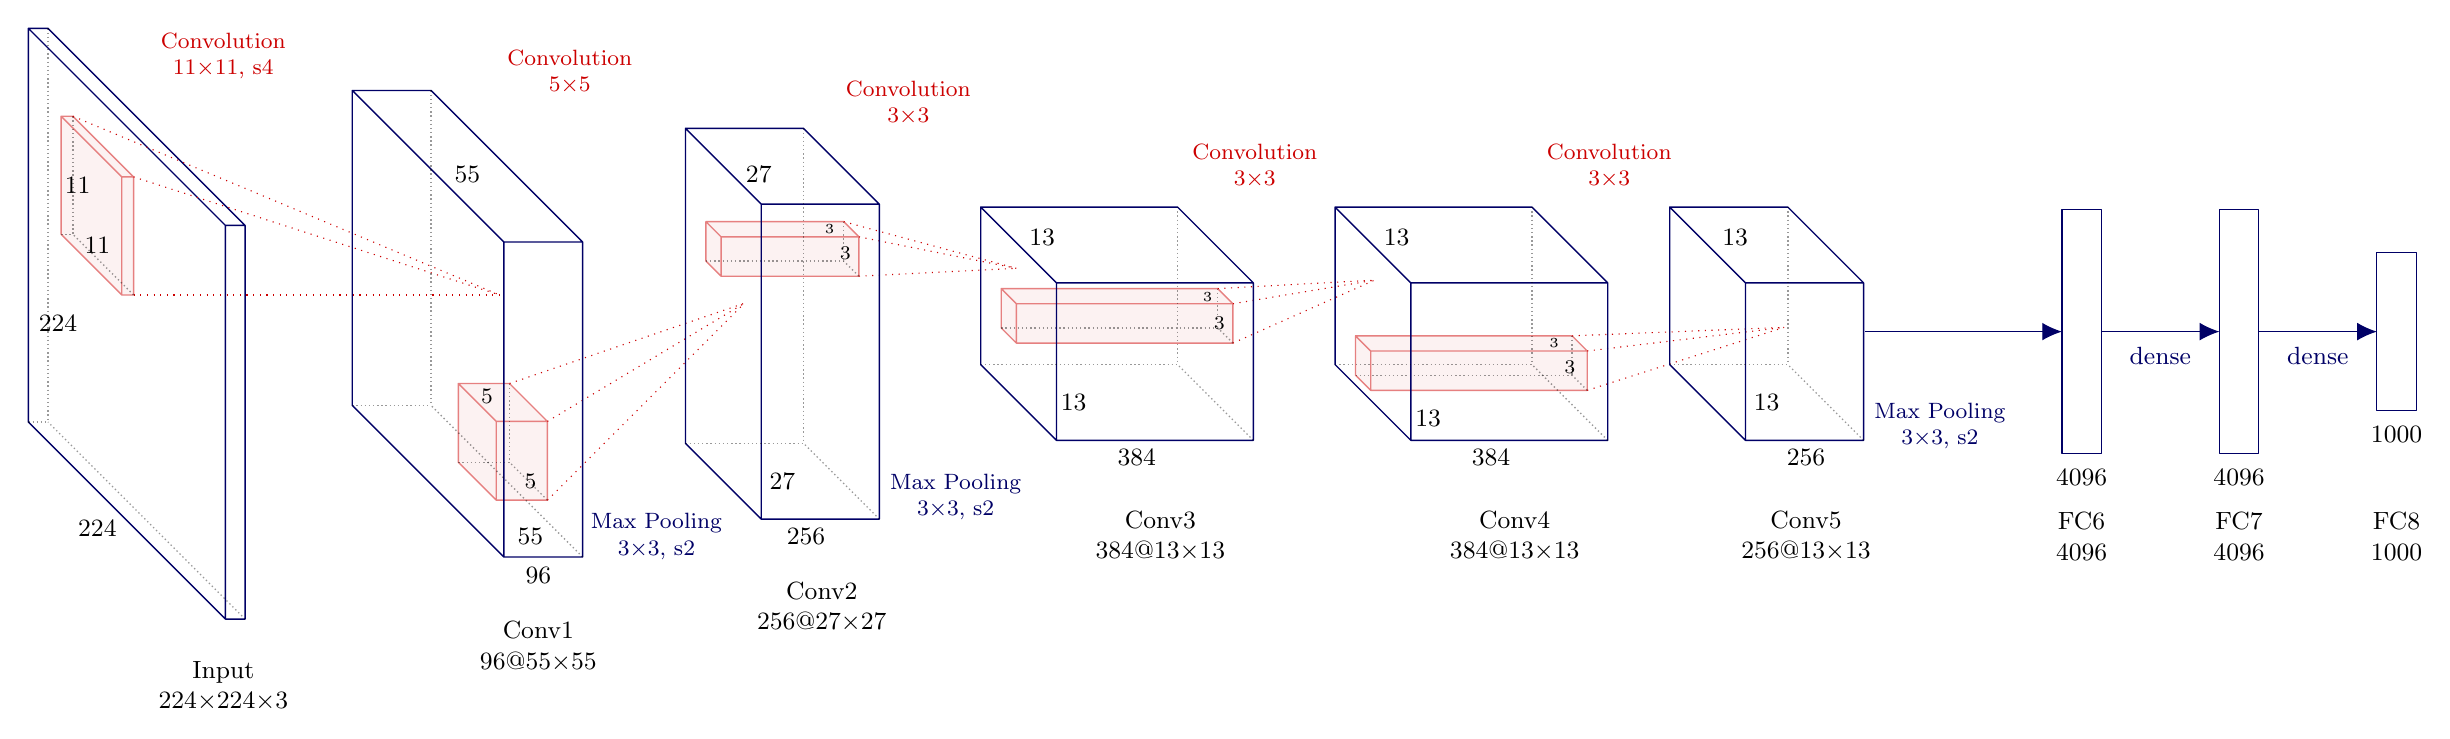
\begin{tikzpicture}[
    font=\small, scale=1, line join=round,
    every node/.style={outer sep=0pt, inner sep=0pt, align=center},
    w/.style={minimum width=#1},
    h/.style={minimum height=#1},
    s/.style={minimum size=#1},
    eu/.style={shorten >=#1},
    ed/.style={shorten <=#1},
    >={Latex[length=2.5mm, width=2.25mm]}
  ]

  % ========== 立方体绘制宏 ==========
  \def\cube#1#2#3#4#5#6#7{%
    \begin{scope}[shift={(#1,#2)},scale=1]
      \pgfmathsetmacro{\cubex}{#4}
      \pgfmathsetmacro{\cubey}{#5}
      \pgfmathsetmacro{\cubez}{#6}
      \draw [draw=black, line width=.5pt,
             every edge/.append style={draw=black, opacity=.4, densely dotted},
             fill=#7, fill opacity=1]
        (\cubex/2,\cubey/2,\cubez/2) coordinate (o)
          -- ++(-\cubex,0,0) coordinate (a)
          -- ++(0,-\cubey,0) coordinate (b)
            edge coordinate [pos=1] (g) ++(0,0,-\cubez)
          -- ++(\cubex,0,0) coordinate (c) -- cycle
        (o) -- ++(0,0,-\cubez) coordinate (d)
          -- ++(0,-\cubey,0) coordinate (e) edge (g) -- (c) -- cycle
        (o) -- (a) -- ++(0,0,-\cubez) coordinate (f) edge (g) -- (d) -- cycle;
      \node[rotate=90, xshift=-2cm, yshift=.165cm] {#3};
    \end{scope}
  }

  % ========== 主体（水平镜像）==========
  \begin{scope}[xscale=-1]

    % ---- 输入图像 + 11x11 卷积核窗口（抬高 3，与主干对齐）----
    \begin{scope}[xshift=0.2cm, yshift=3cm]
      \cube{0}{0}{}{.25}{5}{6.5}{white,draw=mydarkblue}
      \cube{.5}{1.5}{}{.15}{1.5}{2}{myred!5, draw=myred!50}
      \draw[dotted,myred] (a)--coordinate[pos=1] (zz) +(-4.65,-1.5);
      \draw[dotted,myred] (f)--(zz);
      \draw[dotted,myred] (b)--(zz);
    \end{scope}

    % ---- 单排主干 ----
    \begin{scope}[yshift=1cm]
      \cube{-4.45}{.5}{}{.65}{1}{1.25}{myred!5, draw=myred!50}
      \draw[dotted,myred] (a)--coordinate[pos=1] (zz) +(-2.5,1.5);
      \draw[dotted,myred] (f)--(zz);
      \draw[dotted,myred] (b)--(zz);
      \cube{-4}{2}{}{1}{4}{5}{none,draw=mydarkblue}
      %--（只保留一个 5x5 核）
      \cube{-8}{2.95}{}{1.75}{.5}{.5}{myred!5, draw=myred!50}
      \draw[dotted,myred] (a)--coordinate[pos=1] (zz) +(-2,-.4);
      \draw[dotted,myred] (f)--(zz);
      \draw[dotted,myred] (b)--(zz);
      \cube{-8}{2}{}{1.5}{4}{2.5}{none,draw=mydarkblue}
      %--
      \cube{-12.25}{2.1}{}{2.75}{.5}{.5}{myred!5, draw=myred!50}
      \draw[dotted,myred] (a)--coordinate[pos=1] (zz) +(-1.8,.3);
      \draw[dotted,myred] (f)--(zz);
      \draw[dotted,myred] (b)--(zz);
      \cube{-12.25}{2}{}{2.5}{2}{2.5}{none,draw=mydarkblue}
      %--
      \cube{-16.75}{1.5}{}{2.75}{.5}{.5}{myred!5, draw=myred!50}
      \draw[dotted,myred] (a)--coordinate[pos=1] (zz) +(-2.5,.3);
      \draw[dotted,myred] (f)--(zz);
      \draw[dotted,myred] (b)--(zz);
      \cube{-16.75}{2}{}{2.5}{2}{2.5}{none,draw=mydarkblue}
      %--
      \cube{-20.5}{2}{}{1.5}{2}{2.5}{none,draw=mydarkblue}
      %-- 全连接：一条直线
      \node[draw=mydarkblue, w=.5cm, h=3.1cm] (a) at (-24.5,1.9) {};
      \node[draw=mydarkblue, w=.5cm, h=3.1cm] (b) at (-26.5,1.9) {};
      \node[draw=mydarkblue, w=.5cm, h=2cm]  (c) at (-28.5,1.9) {};
      \node[below=2mm of a.south] {4096};
      \node[below=2mm of b.south] {4096};
      \node[below=2mm of c.south] {1000};
      \draw[mydarkblue, <-] (a.west)--+(2.5,0);
      \draw[mydarkblue, ->] (a)--node[below=2mm] {dense} (b);
      \draw[mydarkblue, ->] (b)--node[below=2mm] {dense} (c);
    \end{scope}

  \end{scope}

  % ========== 标题 ==========
  % \node[font=\large] at (13,7.5) {AlexNet (Single GPU)};

  % ========== 操作标签：Convolution（红，顶行）==========
  \node[font=\footnotesize, text=myred] at (0.9,6.4) {Convolution\\11$\times$11, s4};
  \node[font=\footnotesize, text=myred] at (5.3,6.2) {Convolution\\5$\times$5};
  \node[font=\footnotesize, text=myred] at (9.6,5.8) {Convolution\\3$\times$3};
  \node[font=\footnotesize, text=myred] at (14,5) {Convolution\\3$\times$3};
  \node[font=\footnotesize, text=myred] at (18.5,5) {Convolution\\3$\times$3};

  % ========== 操作标签：Max Pooling（蓝，更高一行）==========
  \node[font=\footnotesize, text=mydarkblue] at (6.4,0.3) {Max Pooling\\3$\times$3, s2};
  \node[font=\footnotesize, text=mydarkblue] at (10.2,0.8) {Max Pooling\\3$\times$3, s2};
  \node[font=\footnotesize, text=mydarkblue] at (22.7,1.7) {Max Pooling\\3$\times$3, s2};

  % ========== 尺寸标注 ==========
  % -- 输入部分（随输入上移 3）
  \node at (-0.7,4) {11};
  \node at (-0.95,4.75) {11};
  \node at (-1.2,3) {224};
  \node at (-0.7,0.4) {224};
  % -- 第 1 组
  \node at (4,4.9) {55};
  \node at (4.8,.3) {55};
  \node at (4.9,-.2) {96};
  \node at (4.8,1) {\footnotesize 5};
  \node at (4.25,2.08) {\footnotesize 5};
  % -- 第 2 组
  \node at (7.7,4.9) {27};
  \node at (8.3,.3) {256};
  \node at (8,1) {27};
  \node at (8.6,4.2) {\tiny 3};
  \node at (8.8,3.9) {\scriptsize 3};
  % -- 第 3 组
  \node at (11.3,4.1) {13};
  \node at (12.5,1.3) {384};
  \node at (11.7,2) {13};
  \node at (13.4,3.34) {\tiny 3};
  \node at (13.55,3) {\scriptsize 3};
  % -- 第 4 组
  \node at (15.8,4.1) {13};
  \node at (17,1.3) {384};
  \node at (16.2,1.8) {13};
  \node at (17.8,2.75) {\tiny 3};
  \node at (18,2.45) {\scriptsize 3};
  % -- 第 5 组
  \node at (20.1,4.1) {13};
  \node at (21,1.3) {256};
  \node at (20.5,2) {13};

  % ========== 层名注释（底部一行）==========
  \node[align=center] at (0.9,-1.6) {Input\\224$\times$224$\times$3};
  \node[align=center] at (4.9,-1.1) {Conv1\\96@55$\times$55};
  \node[align=center] at (8.5,-0.6) {Conv2\\256@27$\times$27};
  \node[align=center] at (12.8,0.3) {Conv3\\384@13$\times$13};
  \node[align=center] at (17.3,0.3) {Conv4\\384@13$\times$13};
  \node[align=center] at (21,0.3) {Conv5\\256@13$\times$13};
  \node[align=center] at (24.5,0.3) {FC6\\4096};
  \node[align=center] at (26.5,0.3) {FC7\\4096};
  \node[align=center] at (28.5,0.3) {FC8\\1000};

\end{tikzpicture}
\end{document}